\vspace*{0.3cm} \noindent
\subsubsection{Objetivo}

El objevtivo de este filtro, es tomar una imagen y transformar el color, pero dándole un efecto de iluminación. \newline
Para lograrlo, se toma el valor de un pixel y le agrega un porcentaje alfa de sus pixels vecinos. \newline
Si ese porcentaje es positivo, los pixels claros, se vuelven aún más claros y los oscuros se mantienen igual.\newline

%\[ dst_{(x,y)} = \left\{ \begin{array}{ll}
%        src_{(i,j)} & \mbox{si $i < 2 \vee j < 2 \vee i + 2 \leq tamy \vee j + 2 \leq tamx $}\\
%       pepe & \mbox{si no}\\\\end{array} \right. \]
       
\[ dst_{(i,j)} = \left\{ \begin{array}{ll}
         src_{(i,j)} & \mbox{si $i < 2 \vee j < 2 \vee i + 2 \leq tamy \vee j + 2 \leq tamx  $}\\
        min(max(src_{(i,j)} + var_{(i,j)},0, 255)) & \mbox{si no}\\\end{array} \right. \]       

\vspace*{0.3cm} \noindent

\subsubsection{Desarrollo Implementacion C}

\begin{center}
\textbf{Sintesis de Desarrollo} 
\end{center}

%\newline

\begin{center}
\textbf{Explicación detallada de Implementación}

\end{center}

En esta implementación, inicialmente,se crearon dos punteros de matriz uno correspondiente a src y otro a dst.\newline 
Ademas, 4 enteros llamados $sumargb$, $varr$,$varg$ y $varb$ inicializados en 0 y otro entero $max$ inicializado en 4876875. \newline
Luego, realizamos dos ciclos, uno añidado dentro del otro recorriendo de la forma $'(int\ i = 0;\ i < filas;\ i++)'$ y 
$(int\ j = 0;\ j < cols;\ j\ ++)$.\newline
Dentro del segundo ciclo, creamos dos punteros rgb\_t donde uno apuntará a \newline rgb\_t $*p\_d = (rgb\_t*)\  \&dst\_matrix[i][j*3]$, y el otro
a $rgb\_t *p\_s = (rgb\_t*)\ \&src\_matrix[i][j*3]$.\newline
Posteriormente, chequeamos si nos encontramos recorriendo los bordes de la imagen \newline $(i < 2 || j < 2 || (i + 2) >= filas || (j + 2) >= cols)$,
en caso verdadero, guardamos el puntero p\_s en p\_d $*p_d=*p_s$. \newline
En caso negativo, realizamos lo siguiente:\newline
Primero guardamos en $sumargb$ el valor 0, luego, crearemos dos ciclos, uno añidado del otro recorriendo de la siguiente forma:\newline
$(int\  i\_p = i-2;\  i\_p <= i+2;\  ++i\_p)$ $(int\  j\_p = j-2;\  j\_p <= j+2;\  ++j\_p)$, dentro del ciclo interno,
creamos un rgb\_t $rgb\_t *s\_s = (rgb\_t*)\  \&src\_matrix[i\_p][j\_p*3]$ y posteriormente al entero $sumargb$ le almacenamos la
suma entre los valores r, g y b del rgb\_t s\_s.\newline
Fuera de estos dos ciclos, y aun dentro de la parte falsa del if, realizamos las siguientes operaciones:\newline
Primero, al entero $varb$ le almacenamos el valor b del rgb\_t p\_s multiplicado por $alfa$ (dado como parametro) y por $sumargb$ $varb = (p\_s\rightarrow b * alfa * sumargb);$.\newline
Segundo, al entero $varg$ le almacenamos el valor g del rgb\_t p\_s multiplicado por $alfa$ (dado como parametro) y por $sumargb$ $varg = (p\_s\rightarrow g * alfa * sumargb);$.\newline
Tercero, al entero $varr$ le almacenamos el valor r del rgb\_t p\_s multiplicado por $alfa$ (dado como parametro) y por $sumargb$ $varr = (p\_s\rightarrow r * alfa * sumargb);$.\newline
Luego, a cada uno de estos tres enteros los dividimos por $max$: \newline
$varb = varb/max;
varg = varg/max;
varr = varr/max;$\newline
Y, por ultimo, al valor b del rgb\_t p\_d le almacenamos $MIN(MAX(p\_s\rightarrow b + varb, 0),255)$ donde MIN y MAX son funciones dadas por la catedra, \newline
Al valor g del rgb\_t p\_d le almacenamos $MIN(MAX(p\_s\rightarrow g + varg, 0),255)$,\newline
Al valor r del rgb\_t p\_d le almacenamos $MIN(MAX(p\_s\rightarrow r + varr, 0),255)$.\newline
Damos por finalizada la parte falsa del if.\newline

Estos dos ciclos realizaran $j\_d = cols - 1$  por $i\_d = filas -1$ de itereaciones.\newline
Con lo mencionado, obtenemos el filtro temperature en c correctamente, con los valores que nos pasan como parámetros.\newline

\vspace*{0.3cm} \noindent
\subsubsection{Desarrollo Implementacion en ASM}
En esta implementacion, a diferencia de en Popart y Temperature, no hubieron tantos casos por chequear, sino que trabajamos 
los bordes por un lado, y la parte interna por el otro. \newline
Recorrimos, por columna de la siguiente forma: \newline

$\hspace*{2.2cm}$$mov\  R12D, 0 $; R12D = 0 contador de filas\newline$
$\hspace*{2.8cm}$mov\  R13D, 0 $; R13D = 0 contador de columnas\newline$
$\hspace*{2.8cm}$mov\  R14D, 0 $; R14 es el offset de acceso a la imagen\newline$
$\hspace*{2.8cm}$mov\  EBX, 0 $; EBX = contador de bytes recorridos en fila\newline$
$\hspace*{2.8cm}$.recorrido\_fila:$\newline$
$\hspace*{2.8cm}$cmp\  R13D, EDX $; EDX = cols) si recorrio todas las columnas\newline$
$\hspace*{2.8cm}$je\  .fin$\newline$
$\newline$
$\hspace*{2.8cm}$.recorrido\_columna:$\newline$
$\hspace*{2.8cm}$	cmp\  R12D, ECX $; si recorrio todas las filas (en una columna)\newline$
$\hspace*{2.8cm}$	je\  .siguiente\_columna$\newline$
$\newline$
$\hspace*{2.8cm}; me fijo si es borde o interior\newline$
$\hspace*{2.8cm}$cmp\  R12D, 2$\newline$
$\hspace*{2.8cm}$jl\  .es\_borde$\newline$
$\hspace*{2.8cm}$cmp\  R13D, 2$\newline$
$\hspace*{2.8cm}$jl\  .es\_borde$\newline$
$\hspace*{2.8cm}$mov\  EAX, R12D $; EAX = contador de filas\newline$
$\hspace*{2.8cm}$add\  EAX, 2$\newline$
$\hspace*{2.8cm}$cmp\  EAX, ECX $; (i + 2) >= filas\newline$
$\hspace*{2.8cm}$jge\  .es\_borde$\newline$
$\hspace*{2.8cm}$mov\  EAX, R13D $; EAX = contador de cols\newline$
$\hspace*{2.8cm}$add\  EAX, 2$\newline$
$\hspace*{2.8cm}$cmp\  EAX, EDX$\newline$
$\hspace*{2.8cm}$jge\  .es\_borde$\newline

Inicializamos varios registros en 0 y comparamos si es Menor a 2 la fila y/o la columna, y en caso de ser asi, chequeamos los
bordes así:

$.es\_borde: ; copio la misma imagen$\newline$
$\hspace*{2.8cm}$	xor\  RAX, RAX$\newline$
$\hspace*{2.8cm}$	mov\  EAX, EBX$\newline$
$\hspace*{2.8cm}$	add\  EAX, R14D$\newline$
$\hspace*{2.8cm}$	mov\  R15, [RDI + RAX]$\newline$
$\hspace*{2.8cm}$	mov\  [RSI + RAX], R15D$\newline$
$\newline$
$\hspace*{2.8cm}$.seguir:$\newline$
$\hspace*{2.8cm}$add\  R12D, 1$\newline$
$\hspace*{2.8cm}$add\  R14D, R8D$ ; R14D = R14D + src\_row\_size\newline$
$\hspace*{2.8cm}$jmp\  .recorrido_columna$$\newline$

Estas iteraciones se realizaran hasta que R12D y R13D sean mayores a 2. \newline
Una vez que esto ocurre pasamos a sumar cada color haciendo:\newline

$\hspace*{2.2cm}$$movdqu\  XMM7, XMM0 $\newline$
$\hspace*{2.8cm}$movdqu\  XMM8, XMM0 $\newline$
$\hspace*{2.8cm}$XORPD\  XMM9, XMM9 $\newline$
$\newline$
$\hspace*{2.8cm}$pshufb\  XMM0, [MASK\_1\_COLOR]$\newline$
$\hspace*{2.8cm}$movdqu\  XMM10, XMM0$\newline$
$\hspace*{2.8cm}$punpcklbw\  XMM10, XMM9 $\newline$
$\hspace*{2.8cm}$pshufb\  XMM7, [MASK\_1\_COLORGREEN]$\newline$
$\hspace*{2.8cm}$movdqu\  XMM12, XMM7$\newline$
$\hspace*{2.8cm}$punpcklbw\  XMM12, XMM9$\newline$
$\hspace*{2.8cm}$pshufb\  XMM8, [MASK\_1\_COLORBLUE] $\newline$
$\hspace*{2.8cm}$movdqu\  XMM14, XMM8$\newline$
$\hspace*{2.8cm}$punpcklbw\  XMM14, XMM9 $\newline$
$\hspace*{2.8cm}$paddw\  XMM10, XMM12$\newline$
$\hspace*{2.8cm}$paddw\  XMM10, XMM14$\newline$
$\hspace*{2.8cm}$movdqu\  XMM0, XMM10$\newline
\newline
Primero, nos guardamos en XMM0 los primeros 15 pixeles haciendo $ movdqu\  XMM0, [RDI]$, luego, el valor de XMM0,
lo guardamos en XMM7 y XMM8, limpiamos XMM9 y con 3 mascaras distintas que lo que hacen es ponernos los 5 pixeles rojos adelante y llenar con 0, 
los 5 pixeles azules y llenar con cero y los 5 pixeles verdes y llenar con ceros. \newline
Realizamos la operacion Pshufb con los tres xmm y las mascaras (un xmm con cada mascara) y luego desempaquetamos de byte a word,
usando el xmm9 que habiamos llenado de 0. \newline
El desempaquetado hace que nos queden los valores en word en los registros XMM10, XMM12, XMM14 respectivamente, y luego
los sumamos con PADDW guardando el valor en XMM10. De esta forma obtenemos en word 
$|b0 + g0 + r0|b1 + g1 + r1|b2 + g2 + r2|b3 + g3 + r3|b4 + g4 + r4|$. \newline
Esto lo realizamos 5 veces, quedandonos con los valores en XMM1, 2 ,3,4 y 5. Luego, sumamos estos XMM y nos queda
el valor en XMM3. Proximo a esto, procedemos a sumar los vecinos: \newline

$\hspace*{2.3cm}$$movdqu\ xmm8,\ xmm3$\newline$
$\hspace*{2.8cm}$movdqu\ xmm9,\ xmm3 $\newline$
$\hspace*{2.8cm}$PSRLDQ XMM9, 8d$\newline$
$\hspace*{2.8cm}$paddw\ xmm3,\ xmm9$\newline$
$\newline$
$\hspace*{2.8cm}$movdqu\ xmm9,\ xmm8 $\newline$
$\hspace*{2.8cm}$PSRLDQ XMM9, 6d$\newline$
$\hspace*{2.8cm}$paddw\ xmm3,\ xmm9$\newline$
$\hspace*{2.8cm}$movdqu\ xmm9,\ xmm8$\newline$
$\hspace*{2.8cm}$PSRLDQ XMM9, 4d$\newline$
$\hspace*{2.8cm}$paddw\ xmm3,\ xmm9$\newline$
$\newline$
$\hspace*{2.8cm}$movdqu\ xmm9,\ xmm8 $\newline$
$\hspace*{2.8cm}$PSRLDQ\  XMM9, 2d$\newline$
$\hspace*{2.8cm}$paddw\ xmm3,\ xmm9$\newline$
$\hspace*{2.8cm}$movdqu\ xmm9,\ xmm3$\newline$
$\hspace*{2.8cm}$PSRLDQ\  XMM9, 2d$\newline$
$\hspace*{2.8cm}$PSLLDQ\  XMM9, 2d$\newline$
$\hspace*{2.8cm}$psubw\ xmm3,\ xmm9 $\newline

En esta seccion vamos moviendo bytes a la izquierda, 8 6 4 y 2 asi logramos sumar todos los vecinos en los packs.\newline
Guardamos en R15D el valor alfa, que nos viene por pila en $[RSP + 56]$. Y lo guardamos en XMM15\newline
Procedemos a la multiplicación por alfa:\newline

$\hspace*{2.3cm}$$movdqu\ xmm7,\ xmm3$\newline$
$\hspace*{2.8cm}$XORPD\ xmm9,\ xmm9$\newline$
$\hspace*{2.8cm}$punpcklwd\ xmm7,\ xmm9$\newline$
$\hspace*{2.8cm}$cvtdq2pd\ xmm7,\ xmm7$\newline$
$\hspace*{2.8cm}$cvtdq2pd\ xmm15,\ xmm15$\newline$
$\hspace*{2.8cm}$mulpd XMM7,\ xmm15$\newline$
$\hspace*{2.8cm}$CVTPD2DQ\ xmm7,xmm7$\newline$
$\hspace*{2.8cm}$movdqu\ xmm3,\ xmm7$$\newline$

En esta seccion desempaquetamos de WORD a DWORD y convertimos a Double para multiplicar con alfa, luego lo convertimos a DWORD.
Guardamos en XMMO el valor de XMM6 y nos quedamos con el del medio, por consiguiente pasamos a multiplicar lo que tenemos con SUMARGB 
y dividimos por MAX: \newline
$\hspace*{2.3cm}$$movdqu XMM7, XMM0$\newline$
$\hspace*{2.8cm}$	movdqu XMM8, XMM0 $\newline$
$\hspace*{2.8cm}$	$\newline$
$\hspace*{2.8cm}$	cvtdq2pd\ xmm3,\ xmm3$\newline$
$\newline$
$\hspace*{2.8cm}$	XORPD\  XMM9, XMM9 $\newline$
$\hspace*{2.8cm}	;multiplico blue \newline$
$\hspace*{2.8cm}$	pshufb\  XMM0, [MASK\_1\_COLOR] $\newline$
$\hspace*{2.8cm}$	movdqu\  XMM10, XMM0$\newline$
$\hspace*{2.8cm}$	punpcklbw\  XMM10, XMM9$\newline$
$\hspace*{2.8cm}$	movdqu\ xmm13, XMM10$\newline$
$\hspace*{2.8cm}$	XORPD\ xmm9,\ xmm9$\newline$
$\hspace*{2.8cm}$	punpcklwd\ xmm13,\ xmm9$\newline$
$\hspace*{2.8cm}$	cvtdq2pd\ xmm13,\ xmm13$\newline$
$\hspace*{2.8cm}$	mulpd\ xmm13,\ xmm3$\newline$
$\hspace*{2.8cm}$	movdqu\  XMM1, XMM13$\newline$
$\newline$
$\hspace*{2.8cm}	;multiplico verde
\newline$
$\hspace*{2.8cm}$	pshufb\  XMM7, [MASK\_1\_COLORGREEN] $\newline$
$\hspace*{2.8cm}$	movdqu\  XMM11, XMM7$\newline$
$\hspace*{2.8cm}$	punpcklbw\  XMM11, XMM9$\newline$
$\hspace*{2.8cm}$	$\newline$
$\hspace*{2.8cm}$	movdqu\ xmm13, XMM11$\newline$
$\hspace*{2.8cm}$	XORPD\ xmm9,\ xmm9 $\newline$
$\hspace*{2.8cm}$	punpcklwd\ xmm13,\ xmm9$\newline$
$\hspace*{2.8cm}$	cvtdq2pd\ xmm13,\ xmm13$\newline$
$\newline$
$\hspace*{2.8cm}$	mulpd\ xmm13,\ xmm3$\newline$
$\newline$
$\hspace*{2.8cm}$	movdqu XMM5, XMM13$\newline$
$\newline$
$\hspace*{2.8cm}	;multiplico red\newline$
$\hspace*{2.8cm}$	pshufb\  XMM8, [MASK\_1\_COLORBLUE]$\newline$
$\hspace*{2.8cm}$	movdqu\  XMM12, XMM8$\newline$
$\hspace*{2.8cm}$	punpcklbw\  XMM12, XMM9$\newline$
$\hspace*{2.8cm}$	movdqu\ xmm13, XMM12$\newline$
$\newline$
$\hspace*{2.8cm}$	XORPD\ xmm9,\ xmm9$\newline$
$\hspace*{2.8cm}$	punpcklwd\ xmm13,\ xmm9$\newline$
$\hspace*{2.8cm}$	cvtdq2pd\ xmm13,\ xmm13$\newline$
$\hspace*{2.8cm}$	mulpd\ xmm13,\ xmm3$\newline$
$\hspace*{2.8cm}$	movdqu\  XMM7, XMM13$\newline

En esta parte procedemos a realizar la multiplicacion de cada color por separado con lo que ya teniamos. Desempaquetando,
convirtiendo a double y por finalizado multiplicando quedandonos en el XMM1, 5 Y 7 los valores obtenidos.\newline
Luego, realizamos la division por max:\newline

$\hspace*{2.3cm}$$ movdqu\  XMM11, [MASK\_MAX]$\newline$
$\hspace*{2.8cm}$cvtdq2pd\  XMM11,XMM11$\newline$
$\hspace*{2.8cm}$divpd\  XMM1, XMM11 $\newline$
$\hspace*{2.8cm}$cvttpd2dq\  XMM1,XMM1 $\newline$
$\hspace*{2.8cm}$packssdw\  XMM1, XMM1$\newline$
$\hspace*{2.8cm}$;GREEN$\newline$
$\hspace*{2.8cm}$divpd\ xmm5,XMM11 $\newline$
$\hspace*{2.8cm}$cvttpd2dq\ xmm5,xmm5$\newline$
$\hspace*{2.8cm}$packssdw\ xmm5,\ xmm5$\newline$
$\hspace*{2.8cm}$;rojo$\newline$
$\hspace*{2.8cm}$divpd\ xmm7,XMM11 $\newline$
$\hspace*{2.8cm}$cvttpd2dq\ xmm7,xmm7$\newline$
$\hspace*{2.8cm}$packssdw\ xmm7,\ xmm7$\newline$
$\newline$
$\hspace*{2.8cm}$movdqu\ xmm9,\ xmm1$\newline$
$\hspace*{2.8cm}$PSRLDQ\  XMM9, 2d$\newline$
$\hspace*{2.8cm}$PSLLDQ\  XMM9, 2d$\newline$
$\hspace*{2.8cm}$psubw\ xmm1,\ xmm9 ;resto para q no me quede basura
$\newline$
$\hspace*{2.8cm}$movdqu\ xmm9,\ xmm5$\newline$
$\hspace*{2.8cm}$PSRLDQ\  XMM9, 2d$\newline$
$\hspace*{2.8cm}$PSLLDQ\  XMM9, 2d$\newline$
$\hspace*{2.8cm}$psubw\ xmm5,\ xmm9 ;resto para q no me quede basura
$\newline$
$\hspace*{2.8cm}$movdqu\ xmm9,\ xmm7$\newline$
$\hspace*{2.8cm}$PSRLDQ\  XMM9, 2d$\newline$
$\hspace*{2.8cm}$PSLLDQ\  XMM9, 2d$\newline$
$\hspace*{2.8cm}$psubw\ xmm7,\ xmm9 ;resto para q no me quede basura
$\newline$
$\hspace*{2.8cm}$;en\ xmm1 tengo blue$\newline$
$\hspace*{2.8cm}$;en\ xmm5 tengo GREEN$\newline$
$\hspace*{2.8cm}$;en\ xmm7 tengo rojo$\newline$
$\hspace*{2.8cm}$; en\ xmm6 me quede con el actual$\newline$
$\hspace*{2.8cm}$movdqu\ xmm15,\ xmm6$\newline$
$\hspace*{2.8cm}$pshufb\ xmm15, [MEQUEDOCONELDELMEDIO]$\newline$
$\hspace*{2.8cm}$movdqu\ xmm8,\ xmm15$\newline$
$\hspace*{2.8cm}$movdqu\ xmm9,\ xmm15$\newline$
$\hspace*{2.8cm}$movdqu\ xmm10,\ xmm15$\newline$
$\hspace*{2.8cm}$pshufb\ xmm8, [MASKCOLORROJO] $\newline$
$\hspace*{2.8cm}$paddw\ xmm8,\ xmm1$\newline$
$\hspace*{2.8cm}$pshufb\ xmm9, [MASKCOLORVERDE]$\newline$
$\hspace*{2.8cm}$paddw\ xmm9,\ xmm5$\newline$
$\hspace*{2.8cm}$pshufb\ xmm10, [MASKCOLORAZUL]$\newline$
$\hspace*{2.8cm}$paddw\ xmm10,\ xmm7$\newline

En esta seccion realizamos la division por max, a diferencia de las otras conversiones, en esta convertimos truncado a double
para no perder presicion en la division. Luego de dividir realizamos distintos shifteos, y proximo a esto, shufteos con mascaras
para ir quedandonos definitivamente con cada color final y sumandolos entre si para proceder a chequear maximos y minimos.\newline
El resultado final lo tenemos en XMM8,9 y 10.\newline

Pasamos a chequear dichos valores:\newline
Primero, chequeando si es mayor a cero: \newline

$\hspace*{2.3cm}$$movdqu\  XMM14,[M0]$\newline$
$\hspace*{2.8cm}$movdqu\ xmm15,xmm0$\newline$
$\hspace*{2.8cm}$pcmpgtw\  XMM15, XMM14$$\newline$

Donde, M0 es una mascara con todos 0. \newline

Y procedemos a:\newline

$\hspace*{2.3cm}$$movdqu\  XMM13,\ xmm0$\newline$
$\hspace*{2.8cm}$	movdqu\ xmm11,\ xmm15  ;$\newline$
$\hspace*{2.8cm}$	pcmpeqw\  XMM14,XMM14 $\newline$
$\hspace*{2.8cm}$	pxor\ xmm11,\ xmm14$\newline$
$\hspace*{2.8cm}$	movdqu\ xmm2, [M0]$\newline$
$\hspace*{2.8cm}$	pand\ xmm2,xmm11$\newline$
$\hspace*{2.8cm}$	pand\ xmm13,\ xmm15$\newline$
$\hspace*{2.8cm}$	movdqu\ xmm1,\ xmm13$\newline

Esto, similar a nuestros chequeos en las implementaciones anteriores de Popart y Temperature, guardamos el valor de la comparación,
realizamos and con los valores chequeados, invertimos el resultado de la comparacion y lo guardamos para que esos casos no vuelvan
a ser chequeados. Luego, nuestro resultado nos queda en XMM1. \newline

Segundo, si el numero es menor a 255: \newline

$\hspace*{2.3cm}$$orpd\ xmm1,xmm2$\newline$
$\hspace*{2.8cm}$movdqu\ xmm0,\ xmm1$\newline$
$\hspace*{2.8cm}$movdqu\  XMM14,[M255]$\newline$
$\hspace*{2.8cm}$movdqu\ xmm15,xmm0$\newline$
$\hspace*{2.8cm}$pcmpgtw XMM14,XMM15$\newline

Donde, M255 es una mascara con todos 255. \newline$\hspace*{2.8cm}$

Procedemos a:\newline

$\hspace*{2.3cm}$$movdqu XMM13,\ xmm0$\newline$
$\hspace*{2.8cm}$	movdqu\ xmm11,\ xmm14  $\newline$
$\hspace*{2.8cm}$	pcmpeqw\  XMM15,XMM15 $\newline$
$\hspace*{2.8cm}$	pxor\ xmm11,\ xmm15$\newline$
$\hspace*{2.8cm}$	movdqu\ xmm4, [M255]$\newline$
$\hspace*{2.8cm}$	pand\ xmm4,xmm11$\newline$
$\hspace*{2.8cm}$	pand\ xmm13,\ xmm14$\newline$
$\hspace*{2.8cm}$	movdqu\ xmm3,\ xmm13$\newline

Esta seccion, como mencionamos antes, similar a las implementaciones anteriores, guardamos el valor de la comparación,
realizamos and con los valores chequeados, invertimos el resultado de la comparacion y lo guardamos para que esos casos no vuelvan
a ser chequeados. Luego, nuestro resultado nos queda en XMM3. \newline

Por ultimo, en nuestra implementacion, juntamos los resultados, chequeando con un contador si pertenece a verde rojo o todo:\newline

$\hspace*{2.3cm}$$add\  r15, 1$\newline$
$\hspace*{2.8cm}$orps\ xmm3,xmm4$\newline$
$\hspace*{2.8cm}$movdqu\ xmm0,xmm3$\newline$
$\hspace*{2.8cm}$cmp\  r15,1$\newline$
$\hspace*{2.8cm}$je\  .verdes$\newline$
$\hspace*{2.8cm}$cmp\  r15,2$\newline$
$\hspace*{2.8cm}$je\  .rojos$\newline$
$\hspace*{2.8cm}$cmp\  r15,3$\newline$
$\hspace*{2.8cm}$je\  .juntoTodo$$\newline$

$.verdes:$\newline$
$\hspace*{2.8cm}$movdqu\ xmm8,\ xmm0$\newline$
$\hspace*{2.8cm}$movdqu\ xmm0,\ xmm9$\newline$
$\hspace*{2.8cm}$jmp\  .chequeo$\newline$
$\hspace*{2.8cm}$\ 	.rojos:$\newline$
$\hspace*{2.8cm}$movdqu\ xmm9,\ xmm0$\newline$
$\hspace*{2.8cm}$movdqu\ xmm0,\ xmm10$\newline$
$\hspace*{2.8cm}$jmp\  .chequeo$\newline$
$\hspace*{2.8cm}$\ 	.juntoTodo:$\newline$
$\hspace*{2.8cm}$movdqu\ xmm10,\ xmm0$\newline$
$\hspace*{2.8cm}$PSLLDQ\ xmm9, 1d$\newline$
$\hspace*{2.8cm}$PSLLDQ\ xmm10, 2d$\newline$
$\hspace*{2.8cm}$paddb\ xmm8,\ xmm9$\newline$
$\hspace*{2.8cm}$paddb\ xmm8,\ xmm10$\newline$
$\hspace*{2.8cm}$movdqu\ xmm0,\ xmm8$\newline

En esta seccion, como mencionamos, realizamos la suma de todos los xmm de los distintos colores.\newline
Una ves terminado esto, guardamos en la imagen resultante los valores: \newline

\hspace*{2.3cm}$xor\  RAX, RAX$\newline$
$\hspace*{2.8cm}$mov\  EAX, EBX$\newline$
$\hspace*{2.8cm}$add\  EAX, R14D$\newline$
$\hspace*{2.8cm}$xor\  R15, R15$\newline$
$\hspace*{2.8cm}$movd\  R15D, XMM0$\newline$
$\hspace*{2.8cm}$mov\  [RSI + RAX], R15D$$\newline$

Esto, finalmente, se realizará hasta que no queden columnas y filas por verse.



\vspace*{0.3cm} \noindent
\subsubsection{Experimento 1}

  Analizar cuales son las diferencias de performace entre las versiones de C y ASM. 
  Realizar gráficos que representen estas diferencias.
  
\vspace*{0.3cm} \noindent

 En este filtro a diferencia de los anteriores existe un alfa el cual da valores positivos y negativos,
 por ende realizamos mediciones con alfa positivo y negativo.
 \vspace*{0.3cm} \noindent
 
 Realizando nuestras mediciones en la implementacion de C y de ASM de nuestro codigos con alfa positivo 
 obtenemos para disversas resoluciones: \vspace*{0.3cm} \noindent
 
 
 120x56
 
En ASM: 1460376

En C:3431854

 \vspace*{0.3cm} \noindent
200x200

En ASM: 9112044

En C:21743294

 \vspace*{0.3cm} \noindent
512x512

En ASM: 64050524

En C:145683856

 \vspace*{0.3cm} \noindent
1023x767

En ASM :193531520

En C:438512256


  \vspace*{0.3cm}

 Para una mejor representación se realizo un grafico mostrando a simple vista
 las diferencias entre cada tipo de implementacion con dicho alfa.
 \vspace*{0.3cm} \vspace*{0.3cm}
  \begin{center}
 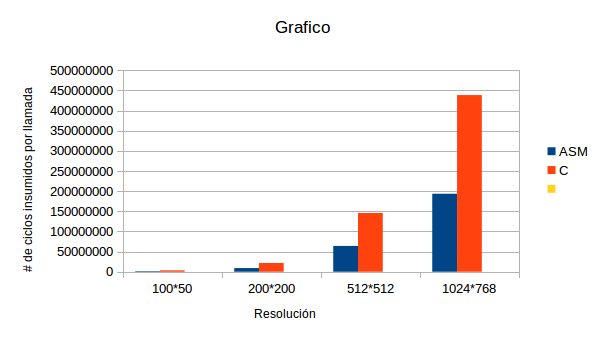
\includegraphics[scale=1]{ldr+.png}
 \end{center}
  \vspace*{0.3cm} 

  Por consiguiente, con un valor alfa negativo realizamos las pertinentes mediciones en las distintas implementaciones 
  obteniendo que: \vspace*{0.3cm} \noindent
  
  
  120x56
  
En ASM: 1438545

En C:3450531

 \vspace*{0.3cm} \noindent
200x200

En ASM: 9026611

En C:21783128

 \vspace*{0.3cm} \noindent
512x512

En ASM: 63927320

En C:145574048

 \vspace*{0.3cm} \noindent
1023x767

En ASM: 193388816

En C:437996160


  
  \vspace*{0.3cm}

 Para una mejor representación se realizo un grafico mostrando a simple vista
 las diferencias entre cada tipo de implementacion con dicho alfa.
 \vspace*{0.3cm} \vspace*{0.3cm}
  \begin{center}
 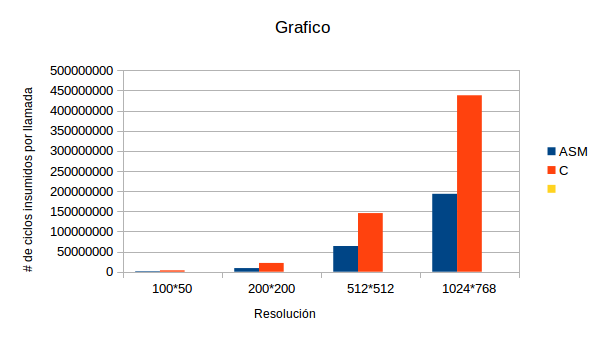
\includegraphics[scale=1]{ldr-.png}
 \end{center}
  \vspace*{0.3cm} 
  
  
La diferencia principal entre el c\'odigo escrito en lenguaje C y el c\'odigo ASM, es la cantidad de accesos 
a memoria realizados en cada iteraci\'on.Otra diferencia puede verse en la cantidad de bytes que pueden 
ser procesados simultaneamente durante el mismo ciclo. En nuestra implamentacion de ASM en una sola iteracion ya
obtenemos la sumas correspondientes de los pixeles vecinos, mientras que en la implamentacion del c por cada iteracion
se realizan dentro de esa misma varias iteraciones mas sumando los pixeles vecinos y por este motivo principal
la diferencia notoria en la performance.\vspace*{0.2cm}

Pudiendo levantar de a 16 bytes en memoria, podr\'ia esperarse que el c\'odigo asm demorase una 
diesiseiava parte de la cantidad de ciclos que demora el c\'odigo en C.
Pero debemos tener en cuenta que en nuestro caso estamos aprovechando solo 15 de los 16 bytes que leemos 
en cada iteraci\'on por lo tanto es más acertado evaluar como si solo leyeramos 15 bytes. 
Adem\'as, hay que tener en cuenta que las instrucciones SSE pueden necesitar más ciclos que las operaciones 
comunes que usamos en el C, eso disminuye un poco la performance en la comparación. 
\vspace*{0.3cm} \vspace*{0.3cm} 
